%%%%%%%%%%%%%%%%%%%%%%%%%%%%%%%%%%%%%%%%%%%%%%%%%%%%%%%%%%%%%%%%%%%%%%%%%%%%%%
%
% Section file included in main project file using \input{}
%
% Assumes that LaTeX2e macros and packages defined in cg_comp.sty are
%   available
%
%%%%%%%%%%%%%%%%%%%%%%%%%%%%%%%%%%%%%%%%%%%%%%%%%%%%%%%%%%%%%%%%%%%%%%%%%%%%%%

 \section{Simple Model of Guitar Intonation\label{sct:model}}
The starting point for prior efforts to understand guitar intonation and compensation~\cite{ref:byers1996cgi,ref:varieschi2010icf} is a formula for $f_{q}$, the transverse vibration frequency harmonic $q$ of a stiff string, originally published by Morse in 1936~\cite{ref:morse1981vsb,ref:fletcher1964nvf, ref:fletcher2005pmb}:
 \begin{equation}\label{eqn:f_m_clamped}
f_{q} = \frac{q}{2\, L}\, \sqrt{\frac{T}{\mu}} \left[ 1 + 2 B + 4 \left(1 + \frac{\pi^2\, q^2}{8}\right) B^2 \right]\, .
 \end{equation}
Here $L$ is the length of the string, $T$ and $\mu$ are its tension and linear mass density, respectively, and $B$ is a small ``bending stiffness'' coefficient to capture the relevant mechanical properties of the string. For a homogeneous string with a cylindrical cross-section, $B$ is given by
 \begin{equation} \label{eqn:b_def}
B \equiv \sqrt{\frac{\pi\, \rho^4\, E}{4\, T\, L^2}}\, ,
 \end{equation}
where $\rho$ is the radius of the string and $E$ is Young's modulus (or the modulus of elasticity). But it's unlikely that \eqn{f_m_clamped} accurately describes the resonant frequencies of a nylon string on a classical guitar, because it assumes that the string is ``clamped'' at both ends, so that a particular set of symmetric boundary conditions must be applied to the partial differential equation (PDE) describing transverse vibrations of the string. We believe that this assumption is correct for the end of the string held at either the nut or the fret, but that the string is ``pinned'' (and not clamped) at the saddle. In \app{freq}, we solve the PDE using these non-symmetric boundary conditions, and find
 \begin{equation} \label{eqn:f_m_stiff}
f_q = \frac{q}{2\, L}\, \sqrt{\frac{T}{\mu}} \left[ 1 + B + \left( 1 + \half q^2 \pi^2 \right) B^2 \right]\, .
 \end{equation}
Note that this expression is valid only when $B \ll 1$. For a typical nylon guitar string with $E \approx 5$~GPa, $T \approx 60$~N, $\rho \approx 0.5$~mm, and $L \approx 650$~mm, we have $B \approx 3 \times 10^{-3}$. (In this case, the quadratic $B$ term in \eqn{f_m_stiff} is only 2\% as large as the linear term, and can generally be neglected. We will include it in our analysis below only for completeness.) We should use \eqn{f_m_stiff} with some caution, because the chemistry, materials science, and physics of nylon strings (particularly the wound bass strings) are quite complicated~\cite{ref:lynchaird2017mpn}.

 \begin{figure}
  \centering
  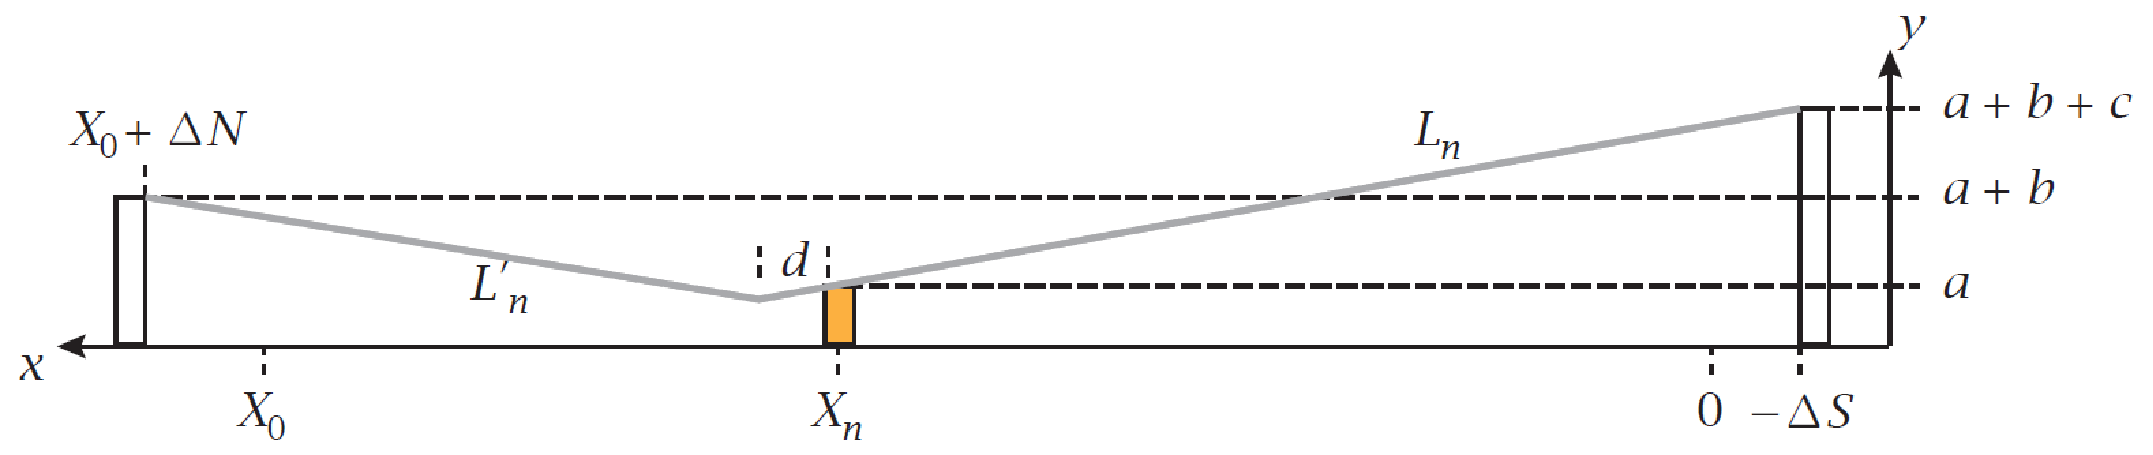
\includegraphics[width=7.0in]{figures/fretting_schematic}
  \caption{\label{fig:guitar_schematic} A simple (side-view) schematic of the classical guitar used in this model. The scale length of the guitar is $X_0$, but we allow the edges of both the saddle and the nut to be set back an additional distance $\Delta S$ and $\Delta N$, respectively. The location on the $x$-axis of the center of the $n^\textrm{th}$ fret is $X_n$. (Note that the $x$-axis is directed toward the left in this figure.) In the $y$ direction, $y = 0$ is taken as the surface of the fingerboard; therefore the height of each fret above the fingerboard is $a$, the height of the nut is $a + b$, and the height of the saddle is $a + b + c$. $L_n$ is the \emph{resonant length} of the string from the saddle to the center of fret $n$, and $L^\prime_n$ is the length of the string from the fret to the nut. We have included a line-segment intersection at a distance $d$ behind fret $n$ to represent the slight increase in the distance $L_n^\prime$ caused by a finger.}
 \end{figure}

Our model is based on the schematic of the guitar shown in \fig{guitar_schematic}. The scale length of the guitar is $X_0$, but we allow the inside edges of both the saddle and the nut to be set back an additional distance $\Delta S$ and $\Delta N$, respectively. The location on the $x$-axis of the center of the $n^\textrm{th}$ fret is $X_n$. In the $y$ direction, $y = 0$ is taken as the surface of the fingerboard; the height of each fret is $a$, the height of the nut is $a + b$, and the height of the saddle is $a + b + c$. (For the time being, we are neglecting the art of \emph{relief} practiced by expert luthiers that adjusts the value of $b$ up the fretboard and strings. We discuss this effect in \sct{comp}.) $L_n$ is the \emph{resonant length} of the string from the saddle to the center of fret $n$, and $L^\prime_n$ is the length of the string from the fret to the nut. The total length of the string is defined as $\mathcal{L}_n \equiv L_n + L^\prime_n$. As discussed in more detail in \app{fret}, we have chosen to include a line-segment intersection at a distance $d$ behind fret $n$ to represent the slight increase in the distance $L_n^\prime$ caused by a finger. This differs from previous studies of guitar intonation and compensation~\cite{ref:byers1996cgi,ref:varieschi2010icf}, but our approach is consistent with empirical observations for nylon strings.

We start with the form of the fundamental frequency of a fretted string given by \eqn{f_m_stiff} with $q = 1$, and apply it to the frequency of a string pressed just behind the $n^\mathrm{th}$ fret:
 \begin{equation} \label{eqn:f_n_def}
f_n = \frac{1}{2\, L_n}\, \sqrt{\frac{T_n}{\mu_n}} \left[ 1 + B_n + \left(1 + \frac{\pi^2}{2}\right) B_n^2 \right]\, ,
 \end{equation}
where $T_n$ and $\mu_n$ are the modified tension and the linear mass density of the fretted string, and
 \begin{equation} \label{eqn:b_n_def}
B_n \equiv \sqrt{\frac{\pi\, \rho^4\, E}{4\, T_n\, L_n^2}}\, .
 \end{equation}
We note that $T_n$ and $\mu_n$ depend on $\mathcal{L}_n$, the \emph{total} length of the fretted string from the saddle to the nut. Ideally, in the 12-TET system~\cite{ref:durfee2015pms},
 \begin{equation} \label{eqn:f_n_tet}
f_n = \gamma_n\, f_0\, , \qquad \textrm{(12-TET~ideal)}
 \end{equation}
where $f_0$ is the frequency of the open (unfretted) string, and
 \begin{equation} \label{eqn:gamme_n_def}
\gamma_n \equiv 2^{n / 12}\, .
 \end{equation}
Therefore, the error interval --- the difference between the fundamental frequency of the fretted string and the corresponding perfect 12-TET frequency --- expressed in cents is given by
 \begin{equation}\label{eqn:error_def}
 \begin{split}
\Delta \nu_n &= 1200\, \log_2\left( \frac{f_n}{\gamma_n\, f_0} \right) \\
%&= 1200\, \log_2 \left( \frac{L_0}{\gamma_n\, L_n}\, \sqrt{\frac{\mu_0}{\mu_n}\, \frac{T_n}{T_0}}\, \frac{1 + B_n}{1 + B_0} \right) \\
&= 1200\, \log_2 \left( \frac{L_0}{\gamma_n\, L_n} \right) + 600\, \log_2 \left(  \frac{\mu_0}{\mu_n} \right) + 600\, \log_2 \left( \frac{T_n}{T_0} \right) \\
&\qquad + 1200\, \log_2 \left[ \frac{1 + B_n + (1 + \pi^2/2)\, B_n^2}{1 + B_0 + (1 + \pi^2/2)\, B_0^2} \right]\, ,
 \end{split}
 \end{equation}
where $\log_2$ is the (binary) logarithm function calculated with base $2$.

The final form of \eqn{error_def} makes it clear that --- for nylon guitar strings --- there are four contributions to intonation:
 \begin{enumerate}
  \item
   \emph{Resonant Length}: The first term represents the error caused by the increase in the length of the fretted string $L_n$ compared to the ideal length $X_n$, which would be obtained if $b = c = d = 0$ and $\Delta S = \Delta N = 0$.
  \item
   \emph{Linear Mass Density}: The second term is the error caused by the reduction of the linear mass density of the fretted string. This effect will depend on the \emph{total} length of the string $\mathcal{L}_n = L_n + L^\prime_n$.
  \item
   \emph{Tension}: The third term is the error caused by the \emph{increase} of the tension in the string arising from the stress and strain applied to the string by fretting. This effect will also depend on the total length of the string $\mathcal{L}_n$.
  \item
   \emph{Bending Stiffness}: The fourth and final term is the error caused by the change in the bending stiffness coefficient arising from the decrease in the vibrating length of the string from $L_0$ to $L_n$.
 \end{enumerate}
Note that the properties of the logarithm function have \emph{decoupled} these physical effects by converting multiplication into addition. We will discuss each of these sources of error in turn below.

In the discussion that follows, we'll test our approximations for a prototypical Classical Guitar with the specifications listed in \tbl{mcg_specs}. Refer to \fig{guitar_schematic} for a graphical representation of these parameters. In addition, as we develop models of the physical effects discussed above, we'll assume that the guitar string has the properties listed in \tbl{string_specs}. The string constant $\kappa$ and the open-string bending stiffness $B_0$ are introduced in \sct{model_tension} and \sct{model_stiffness} respectively. The linear frequency shift parameter $R$ is discussed in \sct{tot_freq_shift}, and a method for determining both $\kappa$ and $B_0$ in terms of $R$ is discussed.

\begin{table}%[htbp]
  \centering
  \caption{\label{tbl:mcg_specs} Default specifications for the prototypical Classical Guitar modeled in this section. The default values of $d$, $\Delta S$, and $\Delta N$ can be either zero or the nonzero value listed in the table and discussed in the text.}
  \begin{tabular}{cll}
    \toprule
    Parameter & Description & Default Value (mm) \\
    \midrule
    $X_0$ & Scale length& $650$ \\
    $b$ & Height of the nut above fret $1$& $1$ \\
    $c$ & Height of the saddle above the nut & $4$ \\
    $d$ & Fretting distance & $0$ or $10$ \\
    $\Delta S$ & Saddle setback & $0$ or $1.9$ \\
    $\Delta N$ & Nut setback & $0$ or $-0.37$ \\
    \bottomrule
  \end{tabular}
\end{table}%

\begin{table}%[htbp]
  \centering
  \caption{\label{tbl:string_specs} Default specifications for a prototypical guitar string. The string constant $\kappa$ and the open-string bending stiffness $B_0$ are introduced in \sct{model_tension} and \sct{model_stiffness} respectively, and the linear frequency shift parameter $R$ is discussed in \sct{tot_freq_shift}.}
  \begin{tabular}{cll}
    \toprule
    Parameter & Description & Default Value \\
    \midrule
    $\rho$ & String radius in mm & $0.43$ \\
    $R$ & Linear frequency shift parameter & $25$ \\
    $\kappa$ & String tension constant & $51$ \\
    $B_0$ & Open-string bending stiffness & $0.00236$ \\
    \bottomrule
  \end{tabular}
\end{table}%

 \subsection{Resonant Length}
The length $L_0$ of the open (unfretted) guitar string can be calculated quickly by referring to \fig{guitar_schematic}. We find:
 \begin{equation}  \label{eqn:l_0_def}
L_0 = \sqrt{\left(X_0 + \Delta S + \Delta N\right)^2 + c^2} \approx X_0 + \Delta S + \Delta N + \frac{c^2}{2\, X_0}\, ,
 \end{equation}
where the approximation arising from the Taylor series is valid to second order in all small distances since $\{\Delta S, \Delta N, b, c\} \ll X_0^2$. Similarly, the resonant length $L_n$ is given by
 \begin{equation}  \label{eqn:l_n_def}
L_n = \sqrt{\left(X_n + \Delta S\right)^2 + (b + c)^2} \approx X_n + \Delta S + \frac{(b + c)^2}{2\, X_n}\, .
 \end{equation}
Then --- if the guitar has been manufactured such that $X_n = X_0 / \gamma_n$ --- the resonant length error determined by the first term in the last line of \eqn{error_def} is approximately
%  \begin{equation}
%  1200\, \log_2 \left( \frac{L_0}{\gamma_n\, L_n} \right) \approx -\frac{1200}{\ln(2)} \left[ \frac{\left(\gamma_n - 1\right) \Delta S - \Delta N}{X_0} + \frac{\gamma_n^2 (b + c)^2 - c^2}{2\, X_0^2}\right]
%  \end{equation}
\begin{equation} \label{eqn:rle_taylor}
  \begin{split}
    1200\, \log_2 \left( \frac{L_0}{\gamma_n\, L_n} \right) &\approx \frac{1200}{\ln(2)} \left[ \frac{\Delta N - \left(\gamma_n - 1\right) \Delta S}{X_0} - \frac{(\Delta N + \Delta S)^2 - \gamma_n^2\, \Delta S^2}{2\, X_0^2}\right. \\ &\qquad\qquad - \left. \frac{\gamma_n^2 (b + c)^2 - c^2}{2\, X_0^2}\right]\, .
  \end{split}
\end{equation}
If the guitar is uncompensated, so that $\Delta S = \Delta N = 0$, the magnitude of this error on our Classical Guitar can be neglected. However, we'll see that choosing $\Delta S > 0$ and $\Delta N < 0$ will allow us to substantially compensate for frequency shift contributions from other effects. In this case, we note that the three terms inside the bracket on the \rhs of \eqn{rle_taylor} are $\{-3.5 \times 10^{-3}, 1.4 \times 10^{-5}, -1.0 \times 10^{-4}\}$, respectively, for the parameter values given by \tbl{mcg_specs}, corresponding to frequency shifts of $\{-6.05, 0.02, -0.17\}$~cents. Therefore, the second two terms are negligible compared to the first, and we can approximate the resonant length error --- for the purposes of estimating setbacks --- as
\begin{equation} \label{eqn:rle_approx}
  1200\, \log_2 \left( \frac{L_0}{\gamma_n\, L_n} \right) \approx \frac{1200}{\ln(2)} \left[ \frac{\Delta N - \left(\gamma_n - 1\right) \Delta S}{X_0}\right]\, .
\end{equation}

 \subsection{Linear Mass Density\label{sct:model_lmd}}
As discussed above, the linear mass density $\mu_0$ of an open (unfretted) string is simply the total mass $M$ of the string clamped between the saddle and the nut divided by the length $L_0$. Similarly, the mass density $\mu_n$ of a string held onto fret $N$ is $M/\mathcal{L}_n$. Therefore
 \begin{equation}
\frac{\mu_0}{\mu_n} = \frac{\mathcal{L}_n}{L_0} \equiv 1 + Q_n\, ,
 \end{equation}
where we have followed Byers and defined the normalized relative displacement~\cite{ref:byers1996cgi,ref:varieschi2010icf}
 \begin{equation} \label{eqn:q_n_def}
Q_n \equiv \frac{\mathcal{L}_n - L_0}{L_0}\, ,
 \end{equation}
where $\mathcal{L}_n = L_n + L_n^\prime$. After judicious use of similar triangles and the Pythagorean Theorem we calculate $L^\prime_n$ for $n \ge 1$ as
\begin{equation} \label{eqn:l_p_def}
  L^\prime_n = \frac{L_n}{X_n + \Delta S}\, d + \sqrt{\left(X_0 - X_n + \Delta N - d\right)^2 + \left(b + \frac{b + c}{X_n + \Delta S}\, d\right)^2}\, .
\end{equation}
In this case, we won't bother with a Taylor series expansion that includes $d \ne 0$, because it isn't significantly more illuminating than \eqn{l_p_def}.

% Since we expect that $Q_n \ll 1$, we can approximate the second term in the final line of \eqn{error_def} as
%  \begin{equation} \label{eqn:lmd_error}
% 600\, \log_2 \left(  \frac{\mu_0}{\mu_n} \right) \approx \frac{600}{\ln(2)}\, Q_n\, .
%  \end{equation}


% Referring to \fig{guitar_schematic}, we see that $\mathcal{L}_n = L_n + L^\prime_n$, and we calculate $L^\prime_n$ for $n \ge 1$ as
%  \begin{equation}
% L^\prime_n = \sqrt{\left(X_0 - X_n + \Delta N\right)^2 + b^2} \approx X_0 - X_n + \Delta N + \frac{b^2}{2 \left(X_0 - X_n\right)}\, ,
%  \end{equation}

However, when $d = 0$, $Q_n$ is approximately
% \begin{equation}
%     \begin{split}
%         L^\prime_n &= \frac{L_n}{X_n + \Delta S}\, d + \sqrt{\left(X_0 - X_n + \Delta N - d\right)^2 + \left(b + \frac{b + c}{X_n + \Delta S}\, d\right)^2} \\
%         &\approx X_0 - X_n + \Delta N + \frac{b^2}{2 \left(X_0 - X_n\right)} + \frac{\left[(b + c)\, X_0 - c\, X_n\right]^2}{2 (X_0 - X_n)^2 X_n^2}\, d
%     \end{split}
% \end{equation}
% to first order in $d/X_0$. Therefore
\begin{equation} \label{eqn:q_n_approx}
  Q_n \approx \frac{\left[ \gamma_n\, b + (\gamma_n - 1)\, c \right]^2}{2\, (\gamma_n - 1)\, X_0^2}\, ,
\end{equation}
accurate to second order in all small distances. This result suggests that the relative displacement does not depend significantly on the setbacks $\Delta S$ and $\Delta N$. In \fig{qn_test}, we plot a comparison between the exact expression for the normalized displacement $Q_n$ given by \eqn{q_n_def} with the approximate expression given by \eqn{q_n_approx} for $d = 0$. Here the guitar has the specifications listed in \tbl{mcg_specs}: the exact expression uses $\Delta S = 1.9$~mm and $\Delta N = -0.37$~mm, and the approximate curve ignores the setbacks entirely. We have also compared \eqn{q_n_def} with both these nonzero and zero setbacks when $d = 10$~mm, and again we see that the dependence of $Q_n$ on the setback values is minimal. We have scaled the relative displacement by a factor of $10^6$ for convenience. For example, at the first fret with $d = 10$~mm, $Q_1 \approx 47 \times 10^{-6}$. This value corresponds to a net stretch of the string at the first fret of $Q_1\, L_0 = 0.03$~mm. Ignoring the setbacks at the $12^{\textrm{th}}$ fret increases $Q_{12}$ by 1\%, a completely negligible amount. For the same parameters, when $d = 10$~mm, $\Delta \nu_{1} \approx 0.04$~cents, and is smaller at all other frets. Therefore, in general the shift due to linear mass density can be neglected without significant loss of accuracy.

% We can use this result and \eqn{q_n_approx} to determine the increase in the relative displacement $Q_n$; we find
%  % \begin{equation} %\label{eqn:delta_q_n_approx}
%  %     \Delta Q_n \approx \left(\frac{\gamma_n}{\gamma_n - 1}\right)^2 \frac{b^2\, d}{2\, X_0^3}\, .
%  % \end{equation}
%  \begin{equation} %\label{eqn:delta_q_n_approx}
%      \begin{split}
%          \Delta Q_n &\approx \frac{\gamma_n^2\, d}{2\, X_0^3} \left( \frac{\gamma_n}{\gamma_n - 1}\, b + c \right)^2 \\
%          &= Q_n\, \frac{\gamma_n^2}{\gamma_n - 1}\, \frac{d}{X_0}\, .
%      \end{split}
%  \end{equation}
% where the approximation applies when $b^2 \ll (X_0 - X_n)^2$. Therefore, using \eqn{l_n_def}, we have
%  \begin{equation}
% \mathcal{L}_n = L_n + L^\prime_n \approx X_0 + \Delta S + \Delta N + \frac{(b + c)^2}{2\, X_n} + \frac{b^2}{2 \left(X_0 - X_n\right)}\, ,
%  \end{equation}
% and
% \begin{equation}
%   \begin{split}
%     Q_n &\approx \frac{1}{2\, X_0} \left[ \frac{(b + c)^2}{X_n} + \frac{b^2}{X_0 - X_n} - \frac{c^2}{X_0} \right] \\
%     &= \frac{\gamma_n}{2\, X_0^2} \left[ (b + c)^2 + \frac{b^2}{\gamma_{n} - 1} - \frac{c^2}{\gamma_n} \right] \\
%     &= \frac{\gamma_n - 1}{2\, X_0^2} \left( \frac{\gamma_n}{\gamma_n - 1}\, b + c \right)^2 \\
%     &= \frac{1}{2\, (\gamma_n - 1)\, X_0^2} \left[ \gamma_n\, b + (\gamma_n - 1)\, c \right]^2 \, .
%  \end{split}
%  \end{equation}

%  \begin{equation} \label{eqn:delta_q_n_approx}
%   \begin{split}
%       \Delta Q_n &\approx \frac{\gamma_n^2\, d}{2\, X_0^3} \left( \frac{\gamma_n}{\gamma_n - 1}\, b + c \right)^2 \\
%       &= Q_n\, \frac{\gamma_n^2}{\gamma_n - 1}\, \frac{d}{X_0}\, .
%   \end{split}
% \end{equation}

% Although it is arguable whether the approximation given by \eqn{q_n_approx} is simpler than the exact expression given by \eqn{q_n_def}, it is quite clear from both \eqn{q_n_approx} and \fig{qn_test} that $Q_n$ \emph{does not depend significantly on the setbacks} $\Delta S$ or $\Delta N$. For the same parameters, when $d = 10$~mm, $\Delta \nu_{1} \approx 0.04$~cents, and is smaller at all other frets. Therefore, in general the shift due to linear mass density can be neglected without significant loss of accuracy.

%If we add this shift due to the linear mass density to the residual quadratic resonant length shift given by \eqn{rle_approx}, then we find the total error
% \begin{equation} \label{eqn:quad_shift}
%\Delta \nu_n = \frac{300}{\ln(2)}\, \frac{\gamma_n}{X_0^2} \left[ \frac{b^2}{\gamma_n - 1} + \frac{c^2}{\gamma_n} - (2 \gamma_n - 1) (b + c)^2 \right]\, .
% \end{equation}
%For the same parameters, $\Delta \nu_{12} = -0.11$~cents, and $|\Delta \nu_n| < |\Delta \nu_{12}|$ for $n < 12$.


\begin{figure}
  \centering
  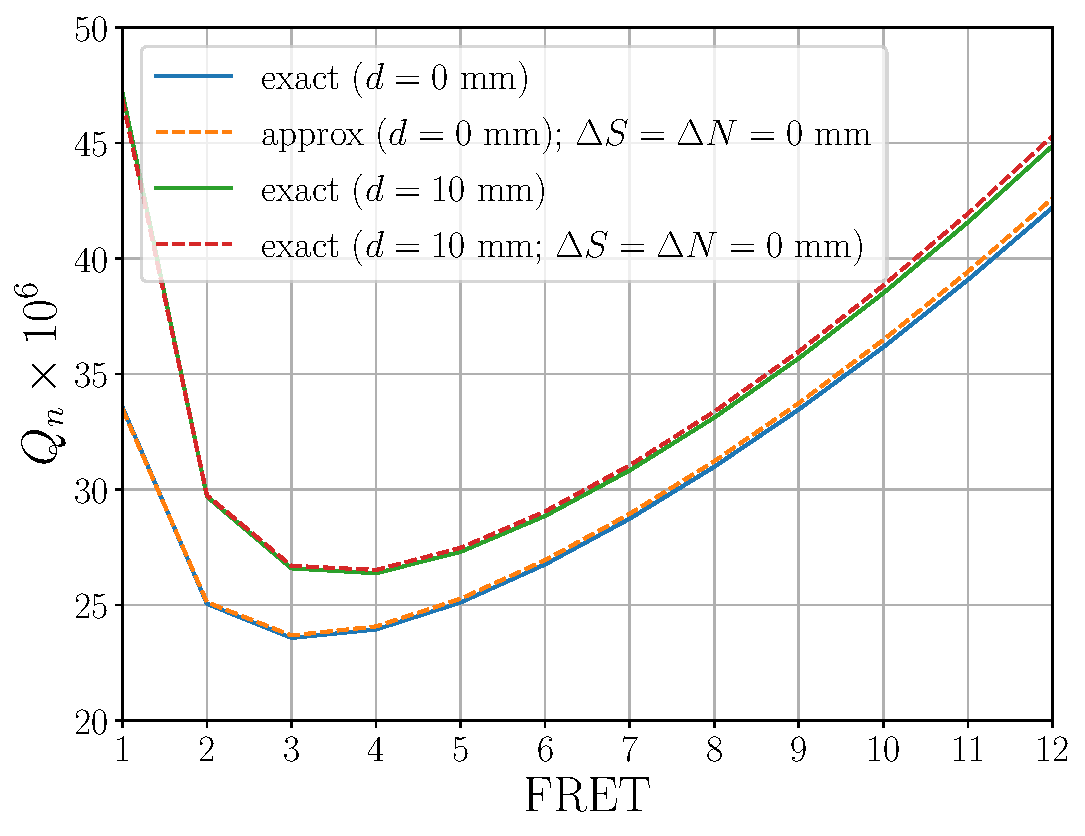
\includegraphics[width=5.0in]{figures/qn_test}
  \caption{\label{fig:qn_test} Comparison of the exact expression for the normalized displacement $Q_n$ given by \eqn{q_n_def} with the approximate expression given by \eqn{q_n_approx}.}
\end{figure}

\begin{figure}
  \centering
  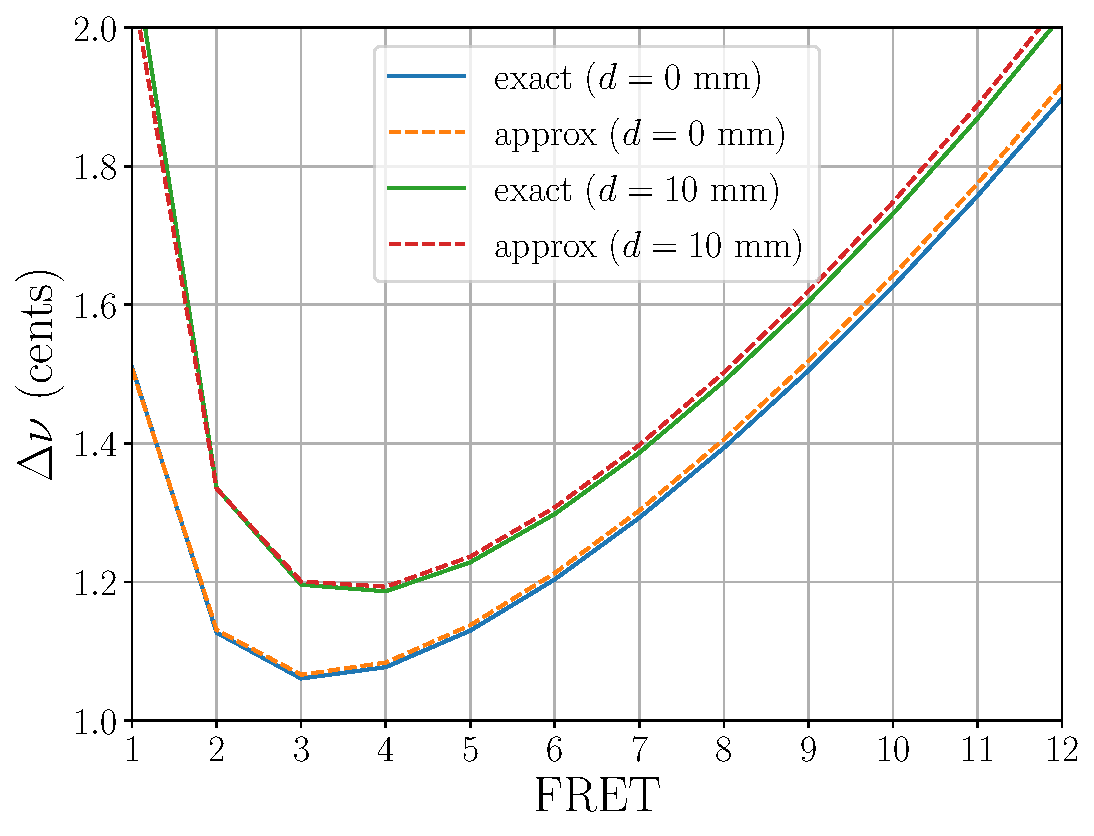
\includegraphics[width=5.0in]{figures/tn_test}
  \caption{\label{fig:tn_test} Comparison of the exact expression for the frequency shift due to tension increases given by the \lhs of \eqn{tension_shift} with the approximate expression given by the right-hand side.}
\end{figure}

 \subsection{Tension\label{sct:model_tension}}
%The third term in \eqn{error_def} provides us withe frequency shift of a string
We've seen above that as a guitar string is fretted its length increases, thereby increasing its tension through linear elastic deformation~\cite{ref:landau1986toe}. We will focus on the response of the string to a longitudinal strain, and neglect the transverse stress that causes negligible changes in the radius of the string~\cite{ref:lynchaird2017mpn}. In this case, we can write the change in tension of a string experiencing an infinitesimal change in length from $L$ to $\mathcal{L}$ as
 \begin{equation} \label{eqn:youngs_mod_def}
\Delta T = \pi\, \rho^2\, E\, \frac{\mathcal{L} - L}{L}\, .
 \end{equation}
Therefore, the tension in a string clamped to fret $n$ is
 \begin{equation} \label{eqn:t_n_def}
T_n = T_0 + \Delta T_n = T_0 \left( 1 + \kappa\, Q_n \right)\, ,
 \end{equation}
where we have used \eqn{q_n_def} and defined the dimensionless linear ``string constant''
 \begin{equation}\label{eqn:kappa_def}
\kappa \equiv \frac{\pi \rho^2 E}{T_0}\, .
 \end{equation}
If we assume that $\kappa\, Q_n \ll 1$, then we can approximate the third term in the final line of \eqn{error_def} as
 \begin{equation} \label{eqn:tension_shift}
600\, \log_2 \left(  \frac{T_n}{T_0} \right) \approx \frac{600}{\ln(2)}\, \kappa\, Q_n\, .
 \end{equation}
This frequency shift is larger than that caused by the linear mass density by a factor of $\kappa$.

In \fig{tn_test}, we compare the exact expression for the frequency shift due to tension increases as a function of the fret number given by the \lhs of \eqn{tension_shift} with the approximate expression given by the \rhs. The exact curves for both $d = 0$~mm and $d = 10$~mm used the corresponding exact expressions for $\mathcal{L}_n$ and $L_0$, while the approximate expressions relied only on \eqn{q_n_approx}. Here we have chosen $\kappa = 51$ from \tbl{string_specs} and the guitar has the same parameters as in \fig{qn_test}.

\subsection{Bending Stiffness\label{sct:model_stiffness}}
% \begin{equation}
%f_{m n} = \frac{m}{2\, L_n}\, \sqrt{\frac{T_n}{\mu_n}} \left( 1 + B_n \right)\, ,
% \end{equation}
The bending stiffness of a string clamped at the $n^{\mathrm{th}}$ fret is given by \eqn{b_n_def}, \eqn{l_n_def}, and \eqn{t_n_def} as
\begin{equation} \label{eqn:bg_n_def}
  B_n = \sqrt{\frac{\pi\, \rho^4\, E}{4\, T_n\, L_n^2}} = \sqrt{1 + \kappa\, Q_n}\, \frac{L_0}{L_n}\, \sqrt{\frac{\pi\, \rho^4\, E}{4\, T_0\, L_0^2}} \approx \gamma_n\, B_0\, ,
\end{equation}
where the approximation applies when $B_0 \ll 1$ and the largest contribution arises from the shortened length of the fretted string compared to that of the open string. This expression confirms our intuitive expectation that the stiffness of the string should increase as the length becomes shorter.
% We see from \eqn{l_n_def} that $L_n \approx L_0/\gamma_n$, so from \eqn{b_n_def} we have
%  \begin{equation} %\label{eqn:bg_n_def}
% B_n = \sqrt{\frac{\pi\, \rho^4\, E}{4\, T_n\, L_n^2}} \approx \frac{L_0}{L_n}\, \sqrt{\frac{\pi\, \rho^4\, E}{4\, T_0\, L_0^2}} = \gamma_n\, B_0\, .
%  \end{equation}
Therefore, the fourth term in the final line of \eqn{error_def} can be approximated as
 \begin{equation} \label{eqn:dnu_bn}
1200\, \log_2 \left[ \frac{1 + B_n + (1 + \pi^2/2)\, B_n^2}{1 + B_0 + (1 + \pi^2/2)\, B_0^2} \right] \approx \frac{1200}{\ln(2)}\, \left[ \left(\gamma_n - 1\right) B_0 + \half\, \left(\gamma_n^2 - 1\right) \left(1 + \pi^2\right) B_0^2 \right]\, .
 \end{equation}
In \fig{stiffness_test}, we use \eqn{bg_n_def} and \eqn{dnu_bn} to compare the exact and approximate expressions for bending stiffness and the corresponding frequency shift based on  \tbl{mcg_specs} and \tbl{string_specs}. Note that we show the approximate frequencies with and without the quadratic terms, and we see that the $2^\mathrm{nd}$-order contribution is about $0.2$~cents at the $12^\mathrm{th}$ fret. Once again, it is clear that $B_n$ does not depend significantly on either $\Delta S$ or $\Delta N$. In other words, the bending stiffness error does not depend on the tiny changes to the linear mass density or the tension that arise due to string fretting. Instead, it is an intrinsic mechanical property of the string: the stiffness increases as the length of the vibrating string becomes shorter.

\begin{figure}
  \centering
  \begin{subfigure}[b]{0.8\textwidth}
      \centering
      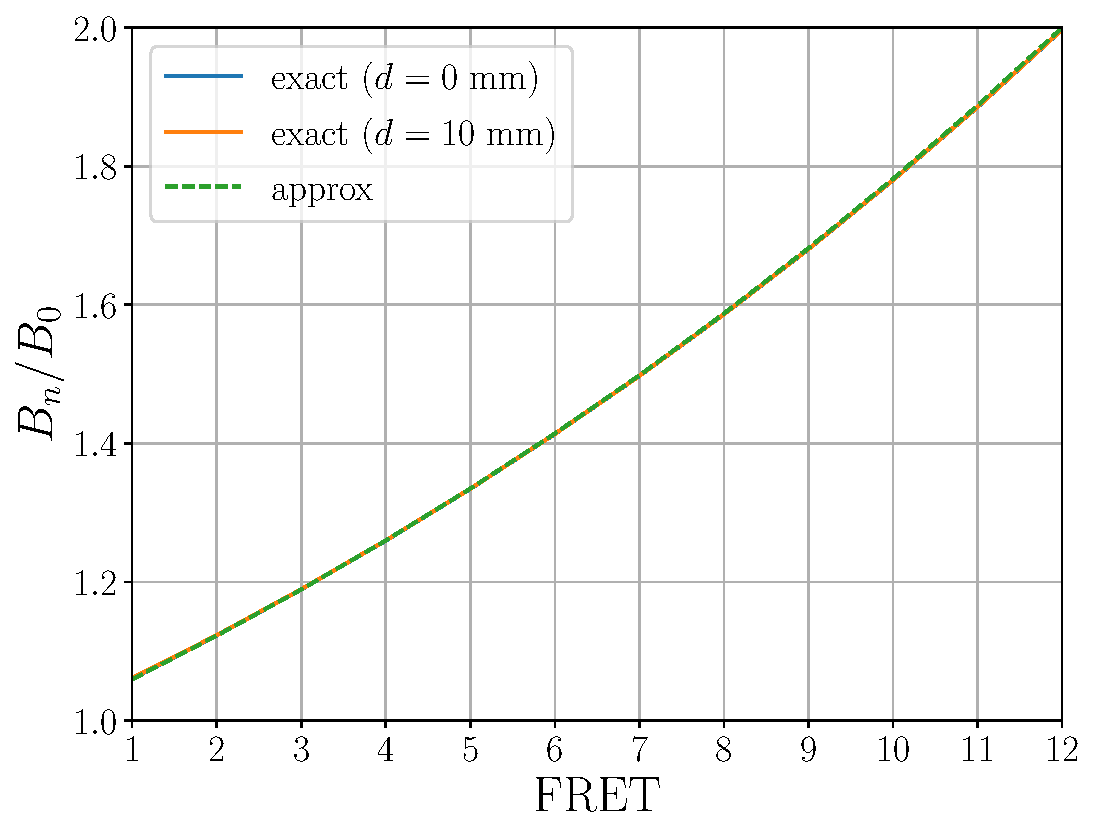
\includegraphics[width=5.0in]{figures/bn_test}
      \caption{Bending stiffness}
      \label{fig:bn_test}
  \end{subfigure}
  \par\vspace{0.25in}
  \begin{subfigure}[b]{0.8\textwidth}
      \centering
      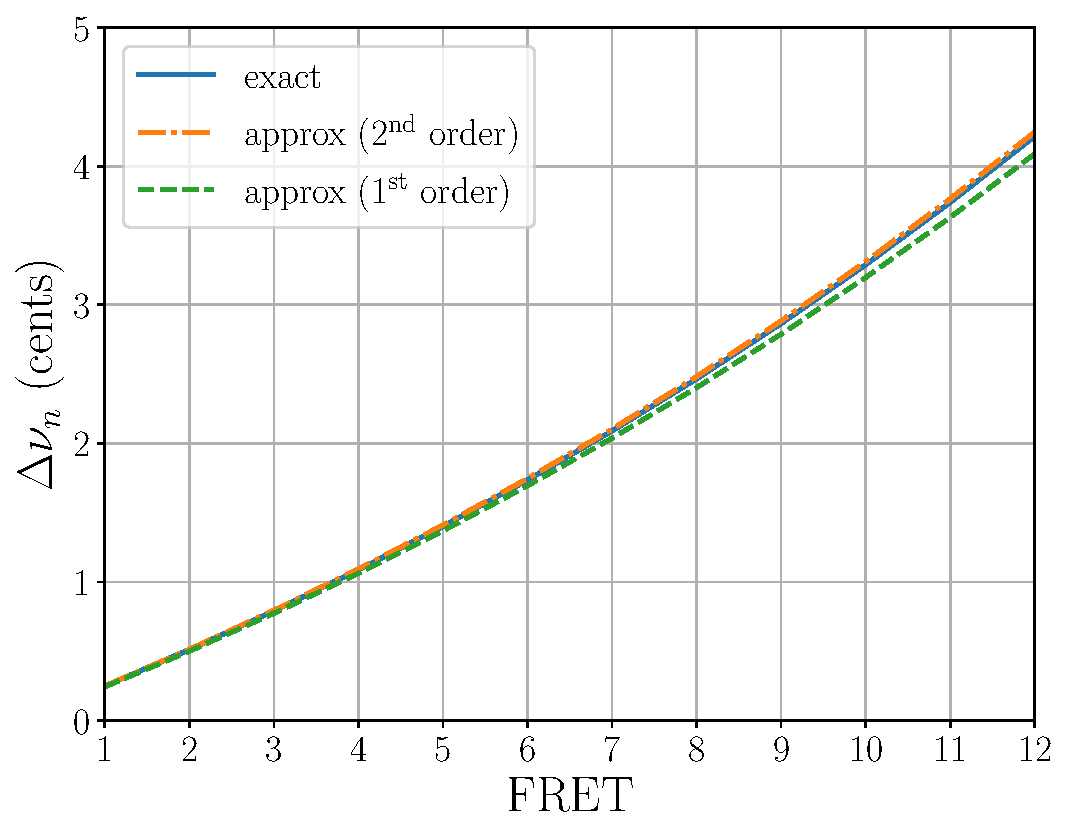
\includegraphics[width=5.0in]{figures/bnu_test}
      \caption{Frequency shifts due to stiffness}
      \label{fig:bnu_test}
  \end{subfigure}
  \caption{\label{fig:stiffness_test} A comparison of exact and approximate expressions for (a) bending stiffness, given by \eqn{bg_n_def}, and (b) the corresponding frequency shift, given by \eqn{dnu_bn}.}
\end{figure}

\subsection{Total Frequency Shift\label{sct:tot_freq_shift}}

Incorporating all of these effects --- and neglecting the term proportional to $B_0^2$ in \eqn{dnu_bn} --- we find that the total frequency shift is given approximately by
\begin{equation}\label{eqn:error_tot}
  \Delta \nu_n \approx \frac{1200}{\ln(2)}\, \left[ \left(\gamma_n - 1\right) \left(B_0 - \frac{\Delta S}{X_0}\right) + \frac{\Delta N}{X_0} + \half\, \kappa\, Q_n \right]\, .
\end{equation}
How do we determine the bending stiffness $B_0$ given by \eqn{b_def} and the spring constant $\kappa$ given by \eqn{kappa_def}? It's impractical to assume that the modulus of elasticity of a particular string can be derived from published values of bulk nylon (particularly in the case of a wound string). Instead, let's assume that we know the value of $\kappa$, and then estimate the bending stiffness coefficient by comparing \eqn{b_def} and \eqn{kappa_def}, and writing $B_0$ as
\begin{equation} \label{eqn:b_0_kappa}
  B_0 = \sqrt{\kappa}\, \frac{\rho}{2\, L_0} \approx \sqrt{\kappa}\, \frac{\rho}{2\, X_0}\, .
\end{equation}

To measure $\kappa$, in \sct{exp} we will conduct an experiment that measures the change in the frequency of an open string --- pinned at one end, and clamped at the other --- as we make slight changes to its length~\cite{ref:byers1996cgi,ref:varieschi2010icf}. From \eqn{f_m_stiff}, the derivative of the fundamental frequency of an open string is
 \begin{equation}
 \begin{split}
\frac{d\, f}{d\, L} &= \frac{f}{L} \left( -1 + \frac{L}{2\, T}\, \frac{d\, T}{d\, L} - \frac{L}{2\, \mu}\, \frac{d\, \mu}{d\, L} + \frac{L}{1 + B}\, \frac{d\, B}{d\, L} \right) \\
&= \frac{f}{L} \left( -1 + \half\, \kappa + \half - \frac{B}{1 + B} \right) \\
&\approx \frac{f}{L} \times \half\, (\kappa - 1)\, ,
 \end{split}
 \end{equation}
where we have used the analyses above to determine that
 \begin{subequations}
 \begin{align}
\frac{d\, T}{d\, L} &= \frac{T}{L}\, \kappa\, , \\
\frac{d\, \mu}{d\, L} &= -\frac{\mu}{L}\, , \nd \\
\frac{d\, B}{d\, L} &= -\frac{B}{L}\, , \\
 \end{align}
 \end{subequations}
and we have again assumed that $B_0 \ll 1$. Therefore, following Byers~\cite{ref:byers1996cgi,ref:varieschi2010icf}, we define the parameter $R$ to be
 \begin{equation}\label{eqn:r_def}
R \equiv \frac{d\, \ln(f)}{d\, \ln(L)} = \frac{L}{f}\, \frac{d\, f}{d\, L} = \half\, (\kappa - 1)\, ,
 \end{equation}
which gives
 \begin{equation} \label{eqn:kappa_r}
\kappa = 2\, R + 1\, .
 \end{equation}

We can estimate the typical value of $R$ for nylon classical guitar strings through a simple observation. On a classical guitar with a scale length of 650~mm, we can usually tune an open string a full step by winding the tuner/machine head three half turns. As we shall see below, this increases or decreases the string length above the first fret by about 3~mm, where the corresponding length of the open string from the saddle to the first fret is about 614~mm. Since a full step is (by definition) 200~cents, \eqn{cents_approx} tells us that
\begin{equation}
  \frac{\Delta f}{f} \approx \frac{\ln(2)}{1200}\, \Delta \nu = \frac{200}{1731} = 0.116\, .
\end{equation}
In this case, we estimate $R$ to be
\begin{equation}
  R \approx \frac{614}{3}\, 0.116 = 24\, ,
\end{equation}
giving $\kappa \approx 49$, close to the values listed in \tbl{string_specs}. The corresponding open-string bending stiffness is computed using \eqn{b_0_kappa} with the scale length given in \tbl{mcg_specs}. In \fig{uncomp}, we plot the total frequency shift given by \eqn{error_def} for this string on the Classical Guitar with $\Delta S = \Delta N = 0$~mm. Note that the string is sharp at every fret, but even a large nonzero value of $d$ is only important at the first fret.

\begin{figure}
  \centering
  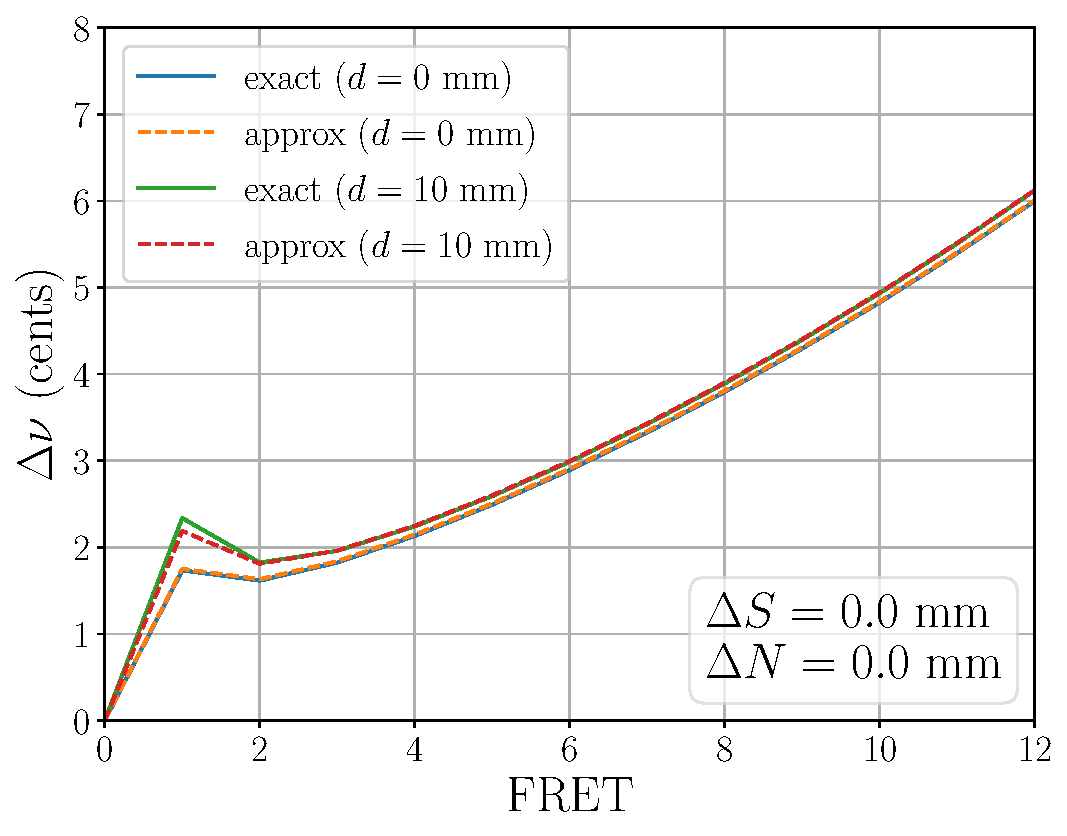
\includegraphics[width=5.0in]{figures/uncomp}
  \caption{\label{fig:uncomp} The total frequency shift given by \eqn{error_def} for the Classical Guitar specified by \tbl{mcg_specs} with $\Delta S = \Delta N = 0$~mm, and a string with the parameters listed in \tbl{string_specs}.}
\end{figure}

\Eqn{error_tot} provides us with a clue on how to modify this guitar to improve the tone of this string. We see that the bending stiffness and the increase in string tension due to fretting sharpen the pitch, but that we can reduce these effects with a positive saddle setback and negative nut setback. In fact, a simple compensation strategy would be to choose
\begin{subequations} \label{eqn:comp_approx}
  \begin{align}
    \Delta S &= B_0\, X_0 \approx \frac{\sqrt{\kappa}}{2}\, \rho\, , \nd \\
    \Delta N &= - \kappa\, X_0\, \overline{Q} / 2\, ,
  \end{align}
\end{subequations}
where we have applied \eqn{b_0_kappa} and defined $\overline{Q}$ as the relative displacement averaged over a particular set of frets to offset string stiffness and tension, respectively.  If we select the first twelve frets, then from \eqn{q_n_approx} with $d = 0$~mm we obtain
\begin{equation} \label{eqn:qbar_approx}
  \overline{Q} \approx \frac{77.9\, b^2 + 35.6\, b\, c + 5.82\, c^2}{24\, X_0^2}\, .
\end{equation}
In the case of the parameters used in \fig{uncomp}, we follow this simple approximate approach to estimate $\Delta S = 1.54$~mm, and $\Delta N = -0.51$~mm. We'll rely on a more accurate method for compensation in \sct{comp}, but we'll obtain results that are similar to those found using this basic approach. In particular, since a \emph{tunable} guitar string has $\sqrt{\kappa} \approx 7.1 \pm 0.3$, we'll discover that the saddle setback is primarily determined by the radius of the string.
